

\section{ Introduction }
\label{intro}

%% problem definition
Obesity is a complex disease involving having too much body fat. Obesity isn't just a cosmetic concern. It's a medical problem that increases the risk of many other diseases and health problems. These can include heart disease, diabetes, high blood pressure, high cholesterol, liver disease, sleep apnea and certain cancers.There are many reasons why some people have trouble losing weight. Often, obesity results from inherited, physiological and environmental factors, combined with diet, physical activity and exercise choices \cite{MayoClinicObesity}. In 2022, 2.5 billion adults aged 18 years and older were overweight, including over 890 million adults who were living with obesity. This corresponds to 43\% of adults aged 18 years and over (43\% of men and 44\% of women) who were overweight; an increase from 1990, when 25\% of adults aged 18 years and over were overweight \cite{WHOObesity}.

Like obesity, underweight can also lead to major health issues. It is regarded as a risk factor that could result in problems including delayed development and weakened immunity. People who are underweight are also more susceptible to infections and other diseases. Treating underweight is crucial for general health, just as obesity is detrimental. A prevalence survey data analysis of the Bangladesh Healthand Demographic Survey in 2014 found that one third (33\%)of the children were underweight in Bangladesh \cite{Hossain2018} 

The purpose of this study is to create a method for checking a person's risk of being overweight or underweight based on their current lifestyle and health choices. By using data on factors like age, gender, eating habits, and exercise levels, the system will use machine learning to find patterns that affect weight-related health problems.

The system will provide personalized feedback on important factors, such as food intake and activity levels, to help users make better choices and take steps to maintain a healthy weight. It will also offer simple advice for healthier eating and exercise routines, making it easier for users to build good habits and reduce the chances of obesity and being underweight in the community.
\section{Background and Present State}
Several research studies have been conducted to analyze factors contributing to obesity and methods for early detection of obesity risks. Some of these studies are discussed in this section. 

In the paper \cite{Islam2022}, the authors focused on the factors related to metabolism that impacted BMI and obesity in adults, using data from the KNHANES survey in Korea. Six machine learning methods were tested: Random Forest, Support Vector Machine, Logistic Regression, Multi-Layer Perceptron, Light Gradient Boosting Machine, and Extreme Gradient Boosting. Among people aged 19–39, the MLP model achieved the best AUC scores, reaching 0.78 for females and 0.77 for males. The RF model attained the highest accuracy, achieving 72\% for males and 76\% for females in this age group. A limitation of the study is that it focused solely on metabolic factors for predicting obesity, without incorporating lifestyle influences. 
In the paper \cite{Sharma2023}, a method was developed for obesity prediction using a machine learning model on a clinical dataset. Five machine learning algorithms were applied: Gradient Boosting, Random Forest, Decision Tree, K-Nearest Neighbor, and Support Vector Machine. GBoost achieved the highest accuracy at 99.05\%, while KNN had the lowest at 95.74\%. Limitations of the paper include not handling class imbalance, which may lower accuracy for smaller groups, and using only clinical data, which may miss important lifestyle factors for predicting obesity. 

In the paper \cite{Raja2023}, a hybrid machine learning approach was developed using a majority voting mechanism, which combined Gradient Boosting Classifier, Extreme Gradient Boosting (XGB), and Multilayer Perceptron (MLP) to predict and classify obesity levels. The approach applied seven algorithms from the UCI dataset and selected the best-performing models, with the hybrid model achieving 97.16\% accuracy. A limitation of this paper is its lack of insight into the specific features influencing weight categories, which restricts its ability to provide personalized recommendations. 

In the paper \cite{Jahan2023}, a method was developed that aimed to classify young Chileans into normal weight, overweight, and obesity categories using machine learning, specifically XGBoost, with biochemical and lipid profile data. The analysis included 21 variables, such as cholesterol, glycemia, and bilirubin, and achieved an accuracy of 87.5\% with an 80\% cross-validation. Limitations of the paper are not considering lifestyle factors as predictors and the lack of multiple levels for obesity stages in the target column, which may reduce the model's depth and accuracy in capturing nuanced obesity risks. 

In the paper \cite{Khan2023}, a machine learning-based system was developed for diet recommendations, focusing on fluid, carbohydrate, protein, and fat intake for patients with non-communicable diseases (NCDs). Six machine learning models were applied: Linear Regression, Support Vector Machine, Decision Tree, Random Forest, XGBoost, and LightGBM. The system achieved the best accuracy using Linear Regression for fluid intake, Random Forest for carbohydrate intake, and LightGBM for protein and fat intake. Explainable AI techniques, such as LIME and SHAP, were employed to improve interpretability. A limitation of this paper is that it doesn’t clearly show which specific factors affect weight categories, which limits its ability to give personalized recommendations. 

In the paper \cite{Nafiseh2023}, the authors suggested a prediction model for obesity risk in 10-year-old children in Korea using logistic regression. The model was based on factors like children's lifestyle habits (e.g., eating regularity, activity levels) and maternal characteristics (e.g., self-esteem, BMI). The final model achieved an accuracy of 74\%. The  limitations of this study include the use of only logistic regression, which may miss complex patterns in the data, and the lack of class-balancing techniques, potentially lowering predictive accuracy for less common categories. 

In the paper \cite{Khalil2023}, a machine learning model is developed to predict obesity risk among overweight individuals, using CatBoost as the primary machine learning model. The model achieved high performance, with an AUC of 0.87 on the test set, and key predictive factors included waist and hip circumferences, female gender, and systolic blood pressure. The limitations are that only CatBoost was tested, which limits model comparison, and the analysis did not consider individuals who are underweight, focusing solely on predicting overweight and obesity. 
\section{Specific Objectives and Possible Outcomes}

The following are the primary objectives of this study: 

\begin{itemize}
    \item To develop a machine learning model capable of predicting the risk of obesity based on current weight and related physical conditions.
    
    \item To use Explainable AI for highlighting the main features contributing to obesity and related health risks.
    
    \item To provide personalized recommendations for users to improve their health outcomes.
    \item  To develop a mobile application that that integrates the machine learning model and recommendation system for user-friendly health management.
\end{itemize}



\section{Outline of Methodology}

The primary objective of this study is to develop a machine learning model that accurately predicts the risk of obesity by identifying key features related to individual physical and lifestyle factors. In addition to prediction, the model will provide personalized recommendations aimed at improving health outcomes. A visual representation of the model’s functionality will be presented in  \ref{methodology}. This holistic approach not only facilitates early detection of obesity risk but also empowers individuals to make informed lifestyle choices, ultimately fostering better public health and well-being. 

% \begin{figure}[!htbp]
%     \centering
%     \includegraphics[width=0.75\textwidth]{figures/workflow.pdf}
%     \caption{Schematic diagram of multi-label aggressive text classification system.}
%     \label{workflow}
% \end{figure}
% % 

\subsection{ Data Collection}
The data for this study will be collected through structured survey-based questionnaires designed to capture a comprehensive range of factors associated with obesity risk. The survey will include inquiries about the respondent's age and gender, daily water intake measured in liters, and the frequency of primary meals consumed each day. It will also gather information on whether vegetables are included in the diet, the quantity of food eaten between meals, and habits related to fast food consumption. Additional questions will cover smoking status and soft drink consumption levels. In addition, the survey will ask about the respondent's physical activity level , the average daily time spent  using digital devices and their primary mode of transportation.The target variable, obesity level, will be determined based on Body Mass Index (BMI) calculations, categorized into five classifications: Underweight, Normal Weight, Obesity Level 1, Obesity Level 2, and Obesity Level 3.This thorough approach to data collection aims to gather diverse and relevant information necessary for developing a machine learning model that accurately predicts obesity risk and offers personalized health recommendations. 

\begin{figure}[!htbp]
    \centering
    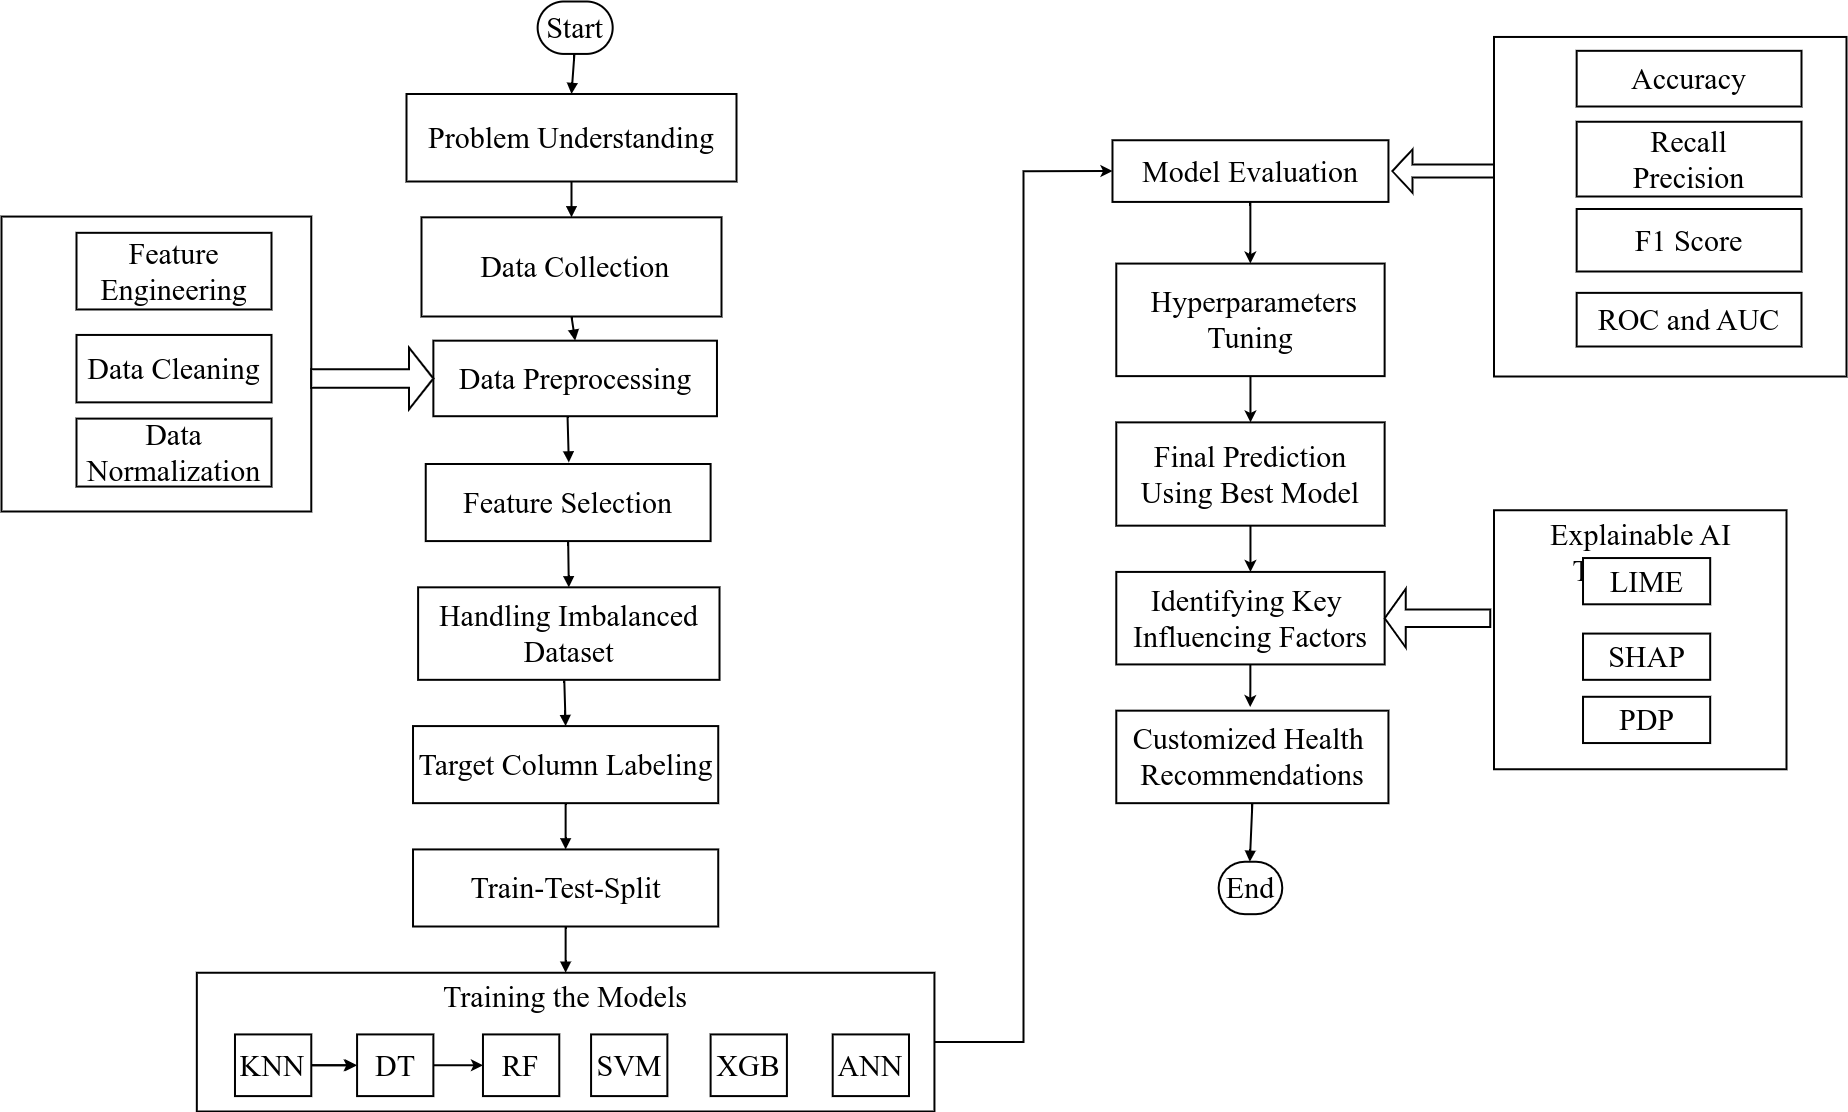
\includegraphics[width=1.0\textwidth]{figures/methodoloy.png}
    
    \vspace{7pt} % Adjust the value (e.g., 5pt, 10pt) to increase spacing
    \caption{Process flow diagram of the proposed methodology.}
    \label{methodology}
\end{figure}


\subsection{Data preprocessing}
Since the data was gathered through a survey, preprocessing is essential before analysis. The initial step will involve checking for any missing values in the dataset. For categorical responses, it will be assumed that if a response is missing, that question is not applicable to the respondent, and this will be handled accordingly. For continuous variables, such as daily water intake and time spent on digital devices, the mean value will be substituted in place of any missing entries.To prepare the data for machine learning, categorical variables will be converted into numerical values. For features without an inherent order, One-Hot Encoding will be applied, while binary variables, such as smoking status or fast food habits, will be handled with Label Encoding. For the transportation mode feature, since it has a natural ranking (where "walking" is best, followed by "public transportation," and then other modes), Ordinal Encoding will be used. This encoding will assign integer values based on priority, ensuring that the model recognizes the ranked preference among transportation options.This preprocessing approach will ensure that the dataset is well-structured and suitable for training accurate predictive models. 
 
 \subsection{Feature Selection}
To determine the most relevant factors contributing to obesity risk, feature selection will be conducted using Pearson Correlation and the Chi-Square test. This approach will help identify features strongly associated with obesity, refining the dataset for better predictive performance and interpretability in line with providing personalized health recommendations. 

\subsection{ Handling Imbalanced Dataset}
To address class imbalance in the dataset, SMOTE (Synthetic Minority Over-sampling Technique) will be applied. SMOTE generates synthetic samples for the minority classes, balancing the dataset without duplicating existing data. This approach aims to improve the model's ability to accurately predict each obesity level, enhancing overall performance and ensuring reliable, inclusive recommendations. 

\subsection{Target Column Labeling}
To prepare the categorical target column, Label Encoding is applied, converting each obesity level into a unique numeric label. This encoding enables the machine learning model to interpret and process the target classes effectively while preserving the categorical distinctions necessary for accurate classification. 

\subsection{Train-Test-Split}
The dataset will be split into three parts: training, validation, and testing. The training set will be used to fit the machine learning model, enabling it to learn from the data. The validation set will then help assess the model's accuracy during training and guide any necessary hyperparameter adjustments to optimize its performance. Finally, the testing set will serve as a final evaluation, providing an unbiased measure of the model’s predictive accuracy and its robustness in identifying obesity risk factors. 
\subsection{Training the Model}

The model will be trained using a combination of advanced machine learning algorithms, including Random Forest, XGBoost, Support Vector Machines (SVM), Artificial Neural Networks (ANN), Decision Trees, and K-Nearest Neighbors (KNN). These algorithms will be evaluated for their performance in predicting obesity levels based on individual physical and lifestyle factors. By leveraging their unique strengths, the training process aims to identify the most effective model for accurate classification. After training, the selected model will undergo validation to ensure its reliability and generalizability in real-world applications. 

 

\subsection{Model Evaluation }

In this study, the performance of the machine learning models will be evaluated using various metrics, including accuracy, recall, precision, and F1 score. These metrics will provide a comprehensive assessment of each model's ability to predict obesity risk. 

\subsection{Hyperparameters Tuning of the Model }

Hyperparameter tuning is a crucial step in optimizing the performance of the selected machine learning model. This process involves adjusting the parameters that govern the learning algorithm to enhance accuracy and reduce overfitting. Techniques such as Grid Search, Random Search, and Bayesian optimization will be employed to systematically explore various combinations of hyperparameters for algorithms like Random Forest, XGBoost, and Artificial Neural Networks (ANN). By identifying the optimal settings for each model, the tuning process aims to improve the model's predictive capabilities, ensuring it generalizes well to unseen data and provides accurate obesity level classifications. 

\subsection{Choosing the Best Model} 

The best model will be selected by comparing various machine learning algorithms based on key evaluation metrics such as accuracy, precision, recall, F1 score, and ROC-AUC. This analysis will help identify the model that most accurately predicts obesity risk. The chosen model demonstrating the highest performance will be selected for final predictions and integrated into the mobile application. 

\subsection{Final Classification}

The best model will be used for the final prediction and to process user input, categorizing each case into the appropriate obesity level based on key physical and lifestyle factors. This prediction will leverage key physical and lifestyle factors, allowing the model to provide accurate insights into the user’s health status. This final classification aims to deliver accurate insights into each user’s health condition. 

 

 

c\subsubsection{Weight Categories }
\begin{itemize}
    \item Underweight 

    \item Normal Weight 

    \item Obesity Levle 1 

    \item Obesity Levle 2 

   \item Obesity Levle 3 
\end{itemize}
\subsection{Identifying Key Influencing Factors }

After predicting the weight category using the optimal model, explainable AI techniques will be utilized to identify key influencing factors that contribute to obesity risk predictions. Techniques such as Permutation Importance, LIME, SHAP, and Partial Dependence Plots (PDP) will be employed to provide insights into how different features impact the model's predictions. This analysis will guide users in understanding which factors play a significant role in their obesity risk, ultimately enabling personalized recommendations for healthier lifestyle choices. 

 

\subsection{Customized Health Recommendations }
The model will offer personalized recommendations by focusing on the important factors that affect obesity and the characteristics of individuals classified as having normal weight in the dataset. By looking for common habits and behaviors among those who maintain a healthy weight, the system will provide simple recommendations that motivate users to adopt similar healthy practices. This approach aims to help users improve their health and make better lifestyle choices to reduce the risk of obesity. 

\section{Mobile Application}

A mobile application will be developed using React Native with Firebase as the database. The app will assess users' lifestyle data to predict their weight category and offer personalized health insights. This intuitive tool aims to empower users in managing their health by providing tailored recommendations based on their unique profiles.

\begin{figure}[H]
    \centering
    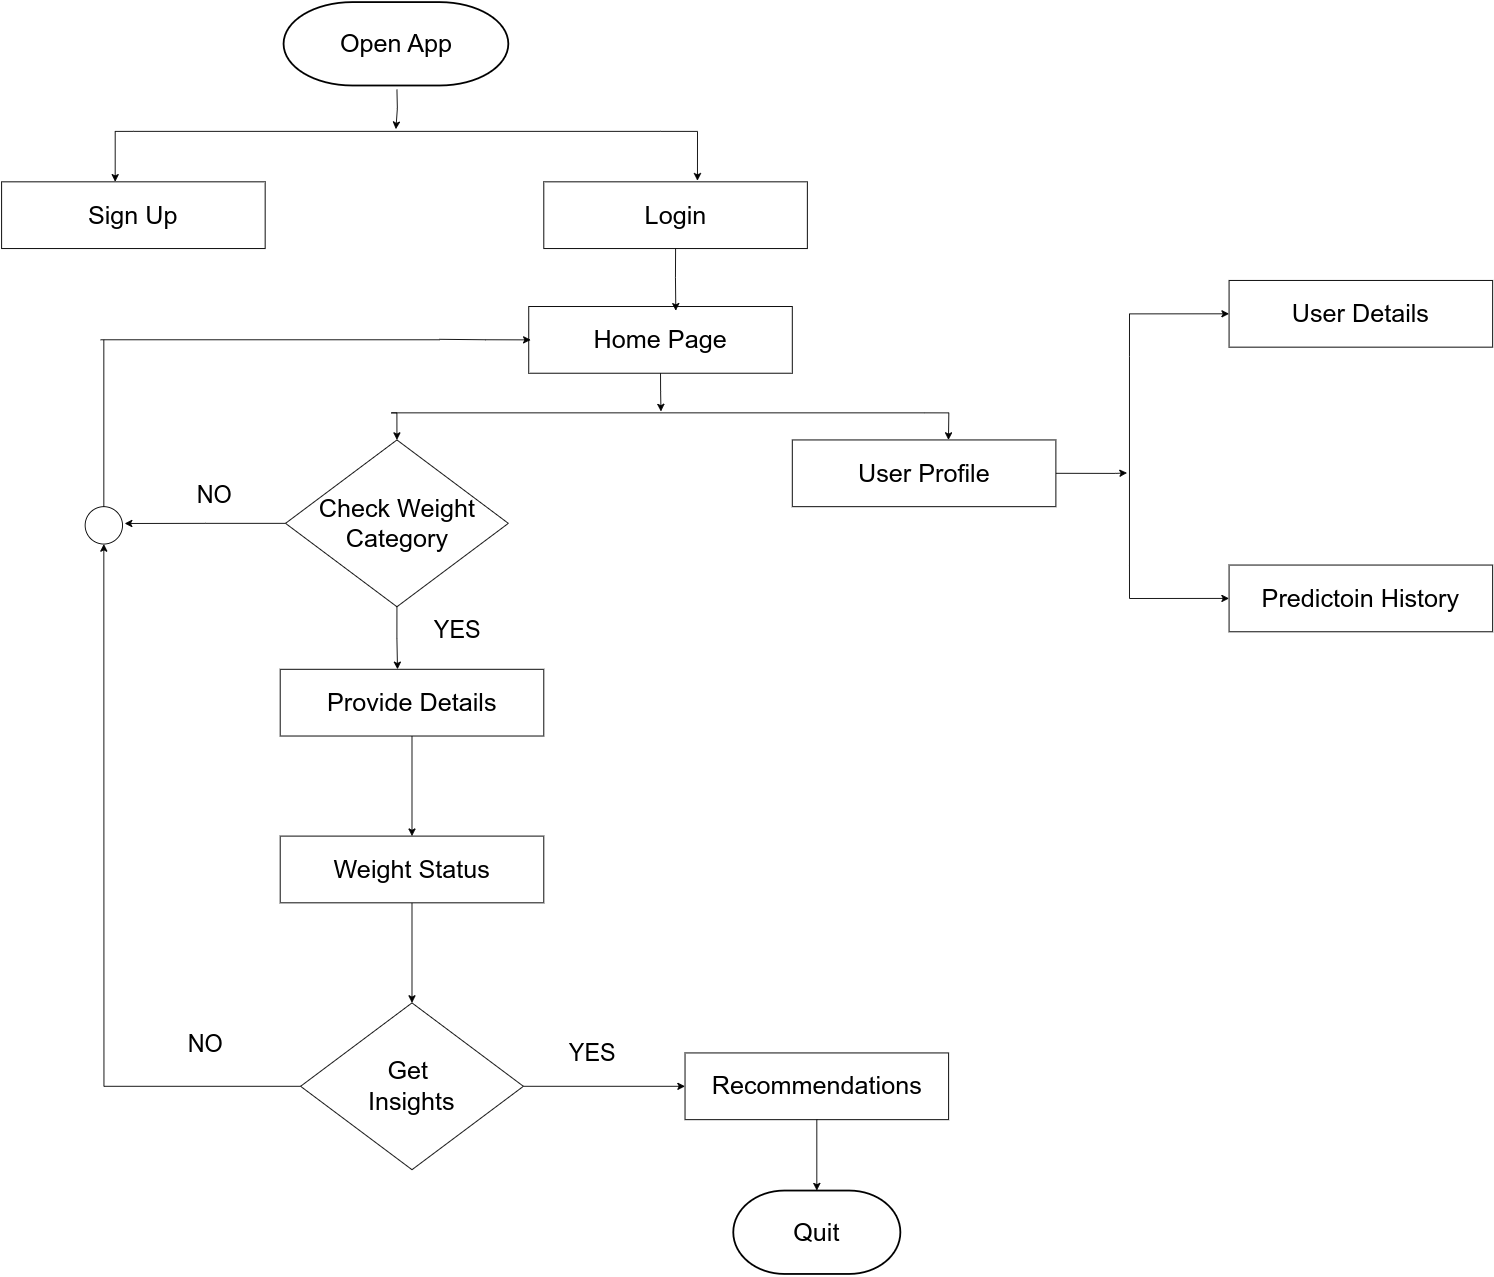
\includegraphics[width=1.0\textwidth]{figures/finalapp.drawio.png}
    
    \vspace{7pt} % Adjust the value (e.g., 5pt, 10pt) to increase spacing
    \caption{Process flow diagram of the Mobile Application.}
    \label{Mobile Application}
\end{figure}
\subsubsection{Features of the Android App}
\begin{itemize}
    \item User Registration: Users can sign up and create a personalized profile.  

    \item Profile Setup: Users can set their age and gender to personalize the experience. 

    \item Lifestyle Data Input: Users can provide lifestyle factors (e.g., diet, activity levels). 

    \item Weight Category Prediction: The system assesses and predicts the user’s weight category. 

   \item Insightful Analysis: Users receive insights into key factors that influenced their weight category prediction. 
   \item Personalized Recommendations: Tailored suggestions help users improve or maintain their health based on the analysis. 
\end{itemize}
\newpage

\section{Required Resources}

Necessary tools and software to implement this project are listed below:

\begin{itemize}
    \item Personal Computer
    \item Jupyter-notebook with Python 3.x installed
\end{itemize}


\section{Cost Estimation}

% Modify from here as necessary for your thesis or project 

\begin{multicols}{2}
    \begin{itemize}
        \item Internet Browsing
        \item Printing and Binding
        \item[Tk] 3000
        \item[Tk] 2000
    \end{itemize}
\end{multicols}

\rule[0pt]{300pt}{1pt} \par
Total \hspace{190pt} Tk. 5000\par
Miscellaneous \hspace{146pt} Tk. 500\par
\rule[0pt]{300pt}{1pt} \par
Grand Total \hspace{157pt} Tk. 5500\par



\newpage

\section{Time Management}
Gantt Chart for the entire approximate timeline from beginning of thesis to the end is added below.
\begin{figure}[th]
\centering
\includegraphics[width=0.9\textwidth]{figures/Gantt chart.pdf}
\caption{Approximate time distribution of thesis }
\label{gantt}
\end{figure}

